%%%%%%%%%%%%%%%%%%%%%%%%%%%%%%%%%%%%%%%%%%%%%%%%%%%%%%%%%%%%%%%%%%%%%%%%%%%%%%%%
% experimental_background.tex: experimental background
%%%%%%%%%%%%%%%%%%%%%%%%%%%%%%%%%%%%%%%%%%%%%%%%%%%%%%%%%%%%%%%%%%%%%%%%%%%%%%%%
% Outline:
% - Motile bacteria sample preparation
% - Video microscopy and image analysis
% - Micro-fabrication and microfluidics
% - Light-controlled E. coli: genetic modification, culturing and trouble shooting
%%%%%%%%%%%%%%%%%%%%%%%%%%%%%%%%%%%%%%%%%%%%%%%%%%%%%%%%%%%%%%%%%%%%%%%%%%%%%%%%


\chapter{Experimental Background}
\label{experimental-background}
%%%%%%%%%%%%%%%%%%%%%%%%%%%%%%%%%%%%%%%%%%%%%%%%%%%%%
In this chapter, experimental techniques that are used in my research will be described briefly as a practical guide for those who want to test or perform some parts of the experiments in this thesis. The following aspects will be covered:
\begin{itemize}
\item \textit{Escherichia coli} (\textit{E. coli}) bacterial suspensions are the model throughout the whole thesis, so I will start talking about the preparation of motile bacterial sample in Sec.~\ref{motile-bacteria-sample-preparation}.
\item A key approach I have been using to investigate the properties of bacterial suspensions is optical microscopy. It is used throughout all the experiments in this thesis as well, along with necessary image analysis techniques. Video microscopy and image analysis will be detailed in
Sec.~\ref{video-microscopy-and-image-analysis-PIV-and-PTV}.
\item When investigating the rheology of bacterial suspensions, we adopted a homemade microfluidic viscometer device. Details of the fabrication are shown in Sec.~\ref{micro-fabrication-and-microfluidics}.
\item A light-powered \textit{E. coli} strain is used in the giant number fluctuations study and the emergence of active turbulence study
(Chap.~\ref{giant-number-fluctuations-in-3-dimensional-space} and Chap.~\ref{the-emergence-of-active-turbulence}). This special strain was obtained by transforming a wild-type strain with an exogenic plasmid which encodes a light-harvesting membrane protein. The discovery and working principles of the light-powering feature has been well documented by earlier works
\cite{Beja2000, Subramanlam2000, DelaTorre2003, Walter2007, Claassens2013}. Following these works, I constructed a plasmid containing the gene and successfully transformed the wild-type \textit{E. coli} strain.
In Sec.~\ref{light-controlled-E-coli-genetic-modification-culturing-and-trouble-shooting}, I will present the details on the materials and procedures I used to construct the mutant as a practical guide to those who need to further modify or trouble shoot the strain I made.
\end{itemize}

\section{Motile Bacteria Sample Preparation}
\label{motile-bacteria-sample-preparation}
Peritrichous \textit{E. coli} bacteria have been widely used as model micro-swimmers for active fluid studies \cite{Poon2012, Schwarz-Linek2016}. By bundling and unbundling their flagella, they achieve a so called ``run-and-tumble'' motion, allowing them to more efficiently explore their surrounding environment and to search for supplies. Fig.~\ref{fig:2-1}a shows a simplified model of a swimming \textit{E. coli} bacterium model with a 2 \textmu m rod-shape body and a helical-shape flagellum of around 8 \textmu m. When swimming, all the flagella bundle together behind the cell and propel it forward \cite{Lauga2015}. Fig.~\ref{fig:2-1}b-c show the bundled state and unbundled state of the flagella, respectively. A swimming \textit{E. coli} bacterium can generate nontrivial fluid flow, which can lead to hydrodynamic attraction to boundaries, alignment with other bacteria and other consequences \cite{Elgeti2015}. It had long been assumed in theoretical works that the effective flow generated by microswimmers like \textit{E. coli} is dipolar, with one force pushing forward from the head and another force pushing backward from the flagella
\cite{Simha2002, Ishikawa2007, Saintillan2008a, Saintillan2008b}. This assumption was then experimentally verified by Drescher et al. in 2011 \cite{Drescher2011}, by reconstructing the flow field from many tracer particle trajectories. Fig.~\ref{fig:2-1}d-e show the flow field they measured and the best-fit force dipole flow. As I will show later, the swimming-induced flow plays a key role in the novel properties and collective motions in the bacterial active fluids.

\begin{figure}[!htbp]
	\begin{center}
	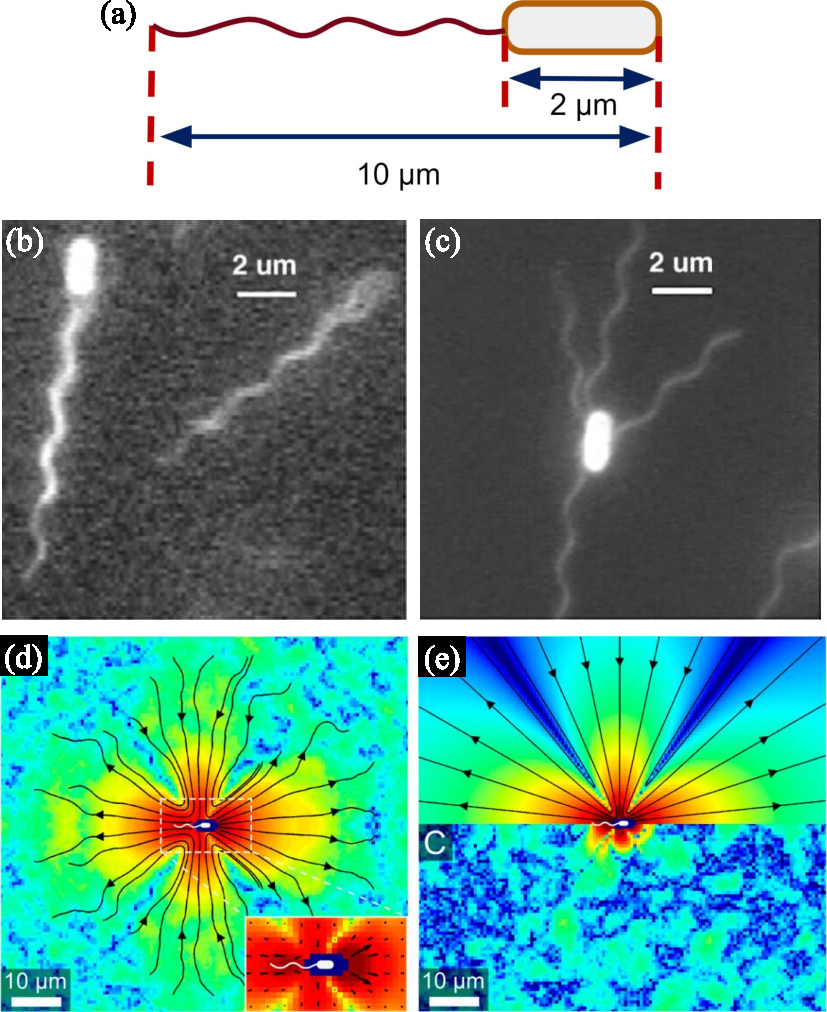
\includegraphics[width=5.5 in]{Figs/2-Exp/1.pdf}
	%select pdftexify command to run jpg or pdf files
	\end{center}
	\caption[Figure 2.1:]
	{
	\textbf{Model swimmer \textit{Escherichia coli} and its flow field.}
  (a) A schematic of a swimming \textit{E. coli} bacterium.
  (b) Fluorescence microscopic image of swimming \textit{E. coli} with bundled flagella.
  (c) Fluorescence microscopic image of tumbling \textit{E. coli} with unbundled flagella.
  (d) Flow field around a swimming \textit{E. coli}, measured with suspending microspheres.
  (e) Best-fit force dipole flow for the flow field shown in (d).
  Image sources:
  (b) and (c) are reproduced from Fig. 4a and 2a in Ref.~\cite{Turner2000} with permission from XXX.
  (d) and (e) are reproduced from Fig. 1a and 1b in Ref.~\cite{Drescher2011} with permission from XXX.
	}
	\label{fig:2-1}
\end{figure}





There are quite a few research groups over the world that are using \textit{E. coli} suspensions to study active fluids. To name a few, Yodh and Arratia at University of Pennsylvania, Wu at Cornell University, Poon at the University of Edinburgh and Clement at ESPCI all have published experimental works using \textit{E. coli} \cite{Chen2007, Patteson2016, Kasyap2014, Jepson2013, Mino2011}. Although the protocols of preparing motile \textit{E. coli} samples are similar across different groups' protocols, they have subtle differences from each other, which may be attributed to the specific strain of \textit{E. coli}, ingredients of media and specific instrument conditions. Schwarz-Linek et al. proposed a sample preparation protocol based on standard bioscience manuals \cite{Bonner2011}
and Berg's \textit{E. coli} protocol. If one wants to learn how to prepare motile \textit{E. coli} from scratch, it is recommended that he/she follows the protocol in Ref.~\cite{Schwarz-Linek2016}.

When I joined the Cheng group at the University of Minnesota in 2015, before Ref.~\cite{Schwarz-Linek2016} was published, there was already a protocol in our lab that worked pretty well for us. I learned the protocol, and have made some modifications over the years to include the additional procedures for preparing light-powered \textit{E. coli} and to optimize the motility and concentration of samples. Below I describe the protocol that works the best in Cheng lab.

\subsection{Background Information}
\begin{description}
  \item [Bacterial strains] We primarily work on two E. coli strains: \textit{AW804} and \textit{BW25113}. \textit{AW804} is light-sensitive. \textit{BW25113} is a wild type strain carrying a plasmid encoding green fluorescence protein, thus it is used when fluorescence / confocal microscopy is needed. Both strains have ampicillin resistance marker and thus require supplementing ampicillin to culturing media.
  \item [Antibiotics] Bacteria are ubiquitous in the environment and can easily  contaminate our bacterial culture. In order to ensure the fidelity of the culture, we add antibiotic resistance markers to the bacteria we want to grow and meanwhile add antibiotics to the medium. The antibiotics inhibit the growth of contaminating species and allow our desired bacteria to grow normally.
  \item [Medium] Various types of media (terrific broth, Luria broth, 2XYT and M9, etc.) are commonly used for bacterial culture. We use terrific broth. The recipe can be found in the protocol section.
\end{description}

\subsection{Protocol}

\begin{enumerate}

  \item Prepare a 2-ml \textit{E. coli} overnight culture.

  \begin{enumerate}
    \item Prepare liquid terrific broth (TB). For example, to make 1 L TB, weigh out the following into a 1 L glass bottle:
    \begin{itemize}
      \item 23.6 g Yeast extract (Sigma-Aldrich)
      \item 11.8 g Tryptone plus (Sigma-Aldrich)
      \item 4 ml Glycerol (XXX)
      \item Add dI water to 1 L
    \end{itemize}
    Loosely close the cap on the bottle (do NOT close all the way or the bottle may explode!) and then loosely cover the top of the bottle with autoclave tape (stick cap and bottle body together to avoid cap popping off). Autoclave and allow to cool to room temperature. Now screw on the top of the bottle and store the TB at room temperature.
    \item Using a sterile 10 ml pipette, transfer 2 ml TB to a sterile glass test tube.
    \item Using a sterile pipette, add 2 microliter (0.1\% v/v) antibiotic solution to the TB in test tube.
    \item Using a sterile pipette tip, pick a small chunk from our bacterial frozen stock (stored in the -80 °C freezer in 251) and carefully transfer the small chunk into the liquid TB + antibiotic.
    \item Loosely cover the culture with sterile cap that is not air tight.
    \item Incubate bacterial culture at 37 °C for 12-18 h in a shaking incubator.
    \item After incubation, check growth, which is characterized by a cloudy haze in the media. This is the overnight culture.
  \end{enumerate}

  \item Dilute overnight culture and harvest motile bacteria at mid-late log phase.
  \begin{enumerate}
    \item Using a sterile 10 ml pipette, transfer 3 ml TB to a sterile glass test tube.
    \item Using a sterile pipette, add 2 microliter (0.1\% v/v) antibiotic solution to the TB in test tube.
    \item Transfer 30 microliter (1\% v/v) overnight culture into the liquid TB + antibiotic.
    \item Incubate bacterial culture at 30 °C for 6-6.5 h in a shaking incubator.
    \item After incubation, check for growth, which is characterized by a cloudy haze in the media. This is the log phase bacteria.
  \end{enumerate}
  \item Centrifuge for better motility and higher concentration bacterial sample.
  \begin{enumerate}
    \item Prepare motility buffer (MB), the following recipe is from Ref.~\cite{Peng2016}.
    \begin{itemize}
      \item 0.01 M potassium phosphate (combine monobasic and dibasic solutions, Sigma-Aldrich)
      \item 10$^{-4}$ M EDTA (Sigma-Aldrich)
      \item 0.002\% weight fraction Tween 20 (Sigma-Aldrich)
      \item Adjust pH to 7.0
    \end{itemize}
    \item Take out the log phase bacteria from the shaking incubator, centrifuge for 5 min at 800 rcf.
    \item Discard the supernatant quickly and transfer the left-over liquid to a new centrifuge tube.
    \item Add 500-1000 ul MB (or water) to resuspend the bottom pellet (avoid bottom pellet) and centrifuge for a second time (5 min, 800 rcf).
    \item Discard the supernatant and let the tubes sit for two minutes. The remaining left-over liquid should be now filled with the active \textit{E. coli}. Take the left-over solution in another capsule and use it for experiments.
    \item To measure the concentration, transfer 10 microliter of the suspension into a 1 ml plastic cuvette and dilute 100 times (by adding 990 microliter water). Put the cuvette in the spectrophotometer in 251 and use the OD600 program. The resulting number times 100 will be the number density of your suspension in the unit of n$_0$ (8 x 10$^8$ cells/ml).
  \end{enumerate}
\end{enumerate}

\begin{figure}[!]
	\begin{center}
	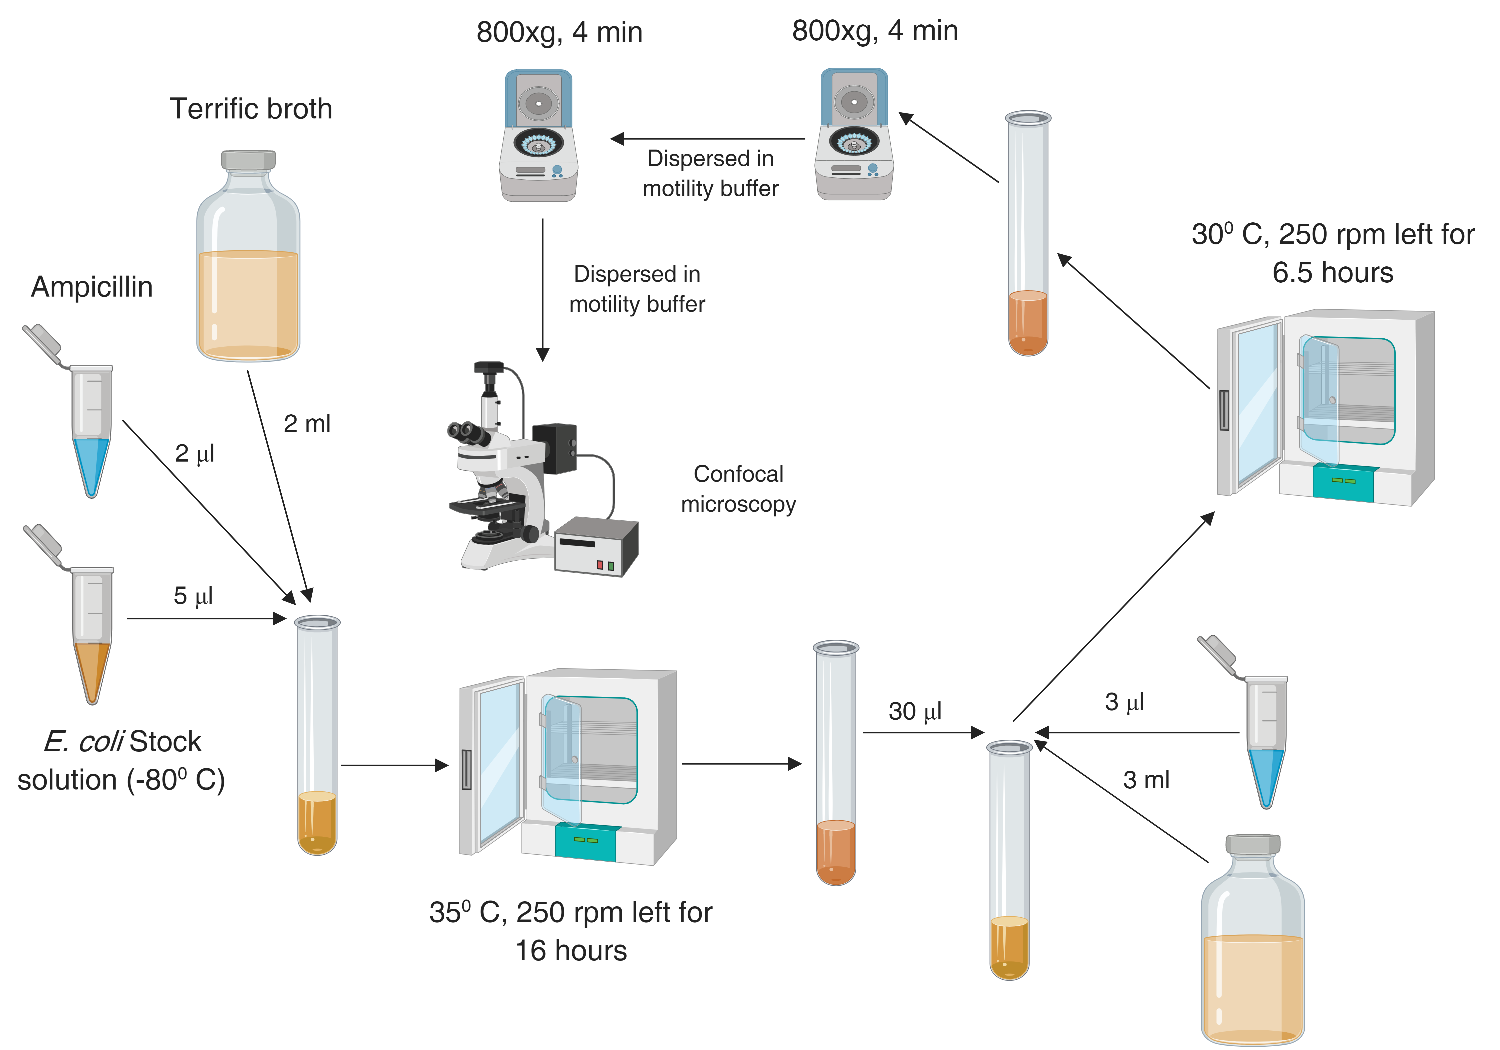
\includegraphics[width=5.5 in]{Figs/2-Exp/2.pdf}
	%select pdftexify command to run jpg or pdf files
	\end{center}
	\caption[Figure 2.2:]
	{
	\textbf{Graphical motile \textit{E. coli} sample preparation protocol.}
	Image courtesy of Shashank Kamdar.
	}
	\label{fig:2-2}
\end{figure}





\section{Video Microscopy and Image Analysis}
\label{video-microscopy-and-image-analysis}
In my experimental research, a standard workflow is
\begin{itemize}
	\item Take videos of samples such as swimming bacteria
	\item Analyze the videos, typically extracting particle position and velocity information from the videos
	\item Calculate from the position and velocity information to obtain more complex information, such as flow field, kinetic energy and diffusivity
\end{itemize}
From this workflow, one can tell that the video microscopy and image analysis are the core skills that enable me to conduct the research.
In this section, I will decribe how I overcome practical challenges when applying these skills in experiments. I want to note that the standard manuals are always the best reference for beginners who have just started to learn about a technique.
In my case, the standard manuals are the Nikon inverted microscope Eclipse Ti-E Ti-E/B instructions \cite{NikonTiEManual}, OpenPIV official website \cite{OpenPIV-website, OpenPIV-paper} and trackpy official website \cite{trackpy-website}.
Some related projects (listed in the websites mentioned) also provide valuable tutorials and ideas, for example the particle tracking routines in IDL by Crocker and Weeks \cite{IDL-tracking} and in Matlab by Blair and Dufresne
\cite{Matlab-tracking}.

\subsection{Video Microscopy}

\subsubsection{Power \textit{E. coli} with Illumination Light}
In the studies of the giant number fluctuations and the emergence of active turbulence, I used a light-powered \textit{E. coli} mutant, which changes its swimming speed according to the amount of light it receives (details of the light-powered \textit{E. coli} mutant can be found in Sec.~\ref{light-controlled-E-coli-genetic-modification-culturing-and-trouble-shooting}).

I use the illumination light of the microscope as the power source of the bacteria, instead of using another light source, based on two considerations: 1) an additional light source shining on the sample will lead to additional unexpected light going into the objective, which often leads to bad image quality; 2) It is hard to construct a spatially uniform light, especially when it has to come in an angle not perpendicular to the specimen. Therefore, I use the illumination light of the microscope to power the \textit{E. coli}.

The light-powered \textit{E. coli} mutant requires quite a high light intensity to move fast enough. Such a high intensity cannot be achieved in the normal microscopy conditions, where four light filters are applied for different purposes. Fig.~\ref{fig:2-3}a-b show the Nikon Ti-E inverted microscope and the illumination light filtering system with the four light filters designated as ND, D, NCB and PFS. The function of the filters are listed below:

\begin{figure}[!htbp]
	\begin{center}
	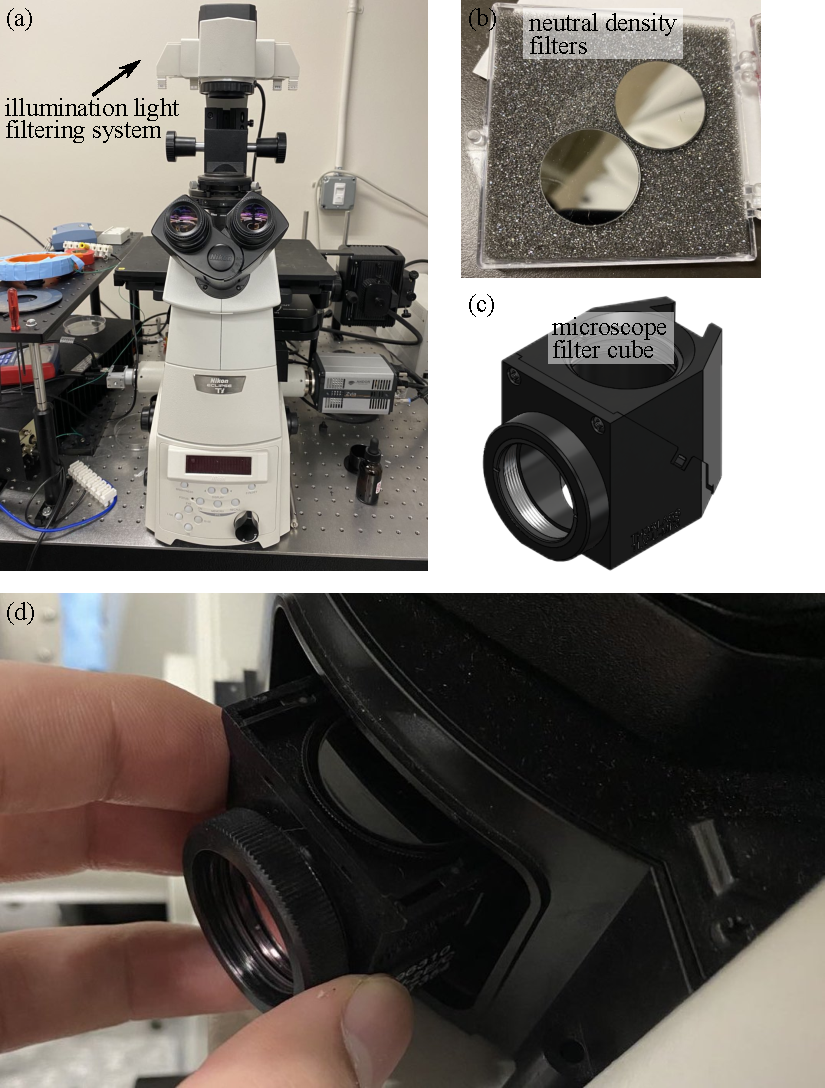
\includegraphics[width=5.5 in]{Figs/2-Exp/3.pdf}
	%select pdftexify command to run jpg or pdf files
	\end{center}
	\caption[Figure 2.3:]
	{
	\textbf{Nikon Ti-E inverted microscope and its filters.}
	(a) Nikon Ti-E inverted microscope model.
	(b) Illumination light path filters.
	(c) Filter block under objective.
	(d) Adding additional ND filter under objective.
	}
	\label{fig:2-3}
\end{figure}

\begin{description}
	\item [ND] Neutral density filter: adjust the brightness for normal microscopy or photomicroscopy
	\item [D] Diffusion filter: made of frosted glass and will diffuse light, used for equalizing the illumination
	\item [NCB] Neutral color balance: corrects the color temperature for mnormal microscopy or filming by daylight type color. Note: this filter is essential for optimal color reproducibility when taking color images, and it should be kept out of the optical path when filming in black and white.
	\item [PFS] Perfect focusing system: a hardware solution to combat axial focus fluctuations in real time during long-term imaging investigations. Note - this filter should be kept out if one does not intend to use the perfect focusing system.
\end{description}

Removing some of those filters can make the illumination light strong enough to power the bacteria. According to the functions of the filters, the only necessary filter is the diffusion filter, given that one is not doing color imaging and is not using perfect focusing system, as it is in my experiment. Fig.~\ref{fig:2-4}a shows an image taken without the diffusion filter (D). Without diffusing the illumination light, the resulting image is clearly inhomogeneous in a large range, with a bright center and a dark bottom area. By putting the diffusion filter in the illumination light path, one can make the illumination light much more uniform, as shown in Fig.~\ref{fig:2-4}b. All the other filters (ND, NCB, PFS) are effectively reducing the overall intensity. Putting in or out these filters only results in globally dimmer or brighter images, without changing the detailed patterns in the image. Thus, these three filters are optional in my experiment. Since powering the light-powered \textit{E. coli} requires a very high light intensity, only the diffusion filter should be kept in the illumination light path.

\begin{figure}[!]
	\begin{center}
	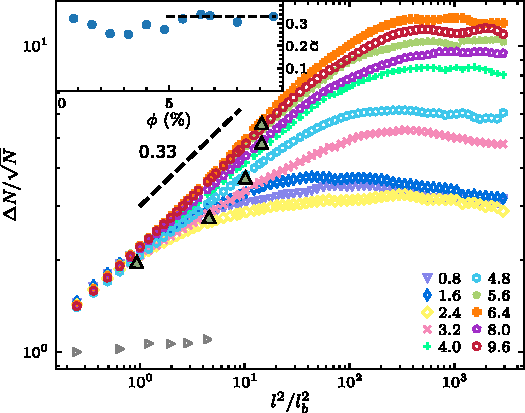
\includegraphics[width=5.5 in]{Figs/2-Exp/4.pdf}
	%select pdftexify command to run jpg or pdf files
	\end{center}
	\caption[Figure 2.4:]
	{
	Image with (a) and without (b) the diffusion filter (D).
	}
	\label{fig:2-4}
\end{figure}





\subsection{Image Analysis}
\subsubsection{Estimate depth of view}








\section{Micro-fabrication and Microfluidics}
\label{micro-fabrication-and-microfluidics}

\section{Light-controlled E. coli: Genetic Modification, Culturing and Trouble Shooting}
\label{light-controlled-E-coli-genetic-modification-culturing-and-trouble-shooting}
